
\subsection{Data}

We used two different datasets to demonstrate the efficacy of \smug.  First, the ever popular, publicly available HC1 dataset\footnote{http://crcns.org/data-sets/hc/hc-1/}
as described in \cite{Henze2000}.  We used the dataset d533101 that consisted of an extracellular tetrode and a single intracellular electrode.  The recording was made simultaneously on all electrodes and was set up such that the cell with the intracellular electrode was also recorded on the extracellular array implanted in the hippocampus of an anesthetized rat. The intracellular recording is relatively noiseless and gives nearly certain firing times of the intracellular neuron.  The extracellular recording contains the spike waveforms from the intracellular neuron as well as an unknown number of additional neurons.  The data is a 4-minute recording at a 10 kHz sampling rate.  

The second dataset comes from Michigan using Michigan probes\footnote{their website perhaps?}.  These data \jovo{@dec - need you here :).}



\jovo{@dec - same pre-processing for both?  regardless, need you to add it.}
We preprocessed with a high-pass filter at 800 Hz before we analyzed the time series.  To get the PCA decomposition, we used the spikes detected with a threshold (three times the standard deviation of the noise above the mean) in the first five seconds and used the top three principal components.  The noise standard deviation was estimated both over the first five seconds of the recording as well as the entire recording, and the estimate was nearly identical.  Our results were also robust to minor variations in the choice of the number of principal components.

Each algorithm gives a clustering of the detected spikes.  In this dataset, we only have a partial ground truth, so we can only verify accuracy for the neuron with the intracellular (IC) recording.  In these experiments, we define a detected spike to be an IC spike if the IC recording has a spike within 0.5 milliseconds (ms) of the detected spike in the extracellular recording.  We define the cluster with the greatest number of intracellular spikes as a the ``IC cluster''.   We refer to these data as ``partial ground truth data'', because we know the ground truth spike times for one of the neurons, but not all the others.  




\subsection{Bake-off Recipes}

We compare a number of variants of \smug, as well as several previously proposed methods, as described below.  The vanilla version of \smug\ operates on a single channel with colored noise.  When using multiple channels, we append an ``\sct{M}'' to obtain \sct{M}\smug.  When we model the mean of the waveforms as an auto-regressive process, we ``post-pend'' to obtain \smug\sct{R}.  
We compare these variants of \smug\ to Gaussian mixture models and k-means with N components (\sct{Gmm-N} and \sct{K-N}, respectively), where \sct{N} indicates the number of components.  Finally, we include a Focus Mixture Model (\sct{Fmm}) \cite{??}, a recently proposed Bayesian generative model with state-of-the-art performance.  Only \smug\ methods were online as we desired to compare to the state-of-the-art \emph{batch} algorithms which use all the data. 
% could not find any previous code available for online spike sorting, despite a small literature on the topic \cite{??}.  
Note that \smug\ algorithms used a dictionary learned from the first five seconds of data, whereas all other algorithms used a dictionary learned from the entire data set.  In either case, the dictionary consisted of the first five principal components of the matrix consisting of all waveforms from the thresholded voltage traces.  Supplementary Figure \ref{fig:waveforms} shows the two different dictionaries and the relative fraction of variance explained.

% 
% 
The single-channel experiments were all run on channel 2 (the results were nearly identical for all channels).  The spike detections for the offline methods used a threshold of three times the noise standard deviation \cite{Lewicki} (unless stated otherwise), and windowed at a size $L=30$.  For multichannel data, we concatenated the $M$ channels for each waveform to obtain a $M\times L$-dimensional vector.
%, and PCA was used to reduce the space to $K$=5 for the experiments. 

% \subsection{Results}


\subsection{Performance on partial ground truth data}



The main empirical result of our contribution is that all variants of \smug\ detect more true positives with fewer false positives than any of the other algorithms on the partial ground truth data (see Figure \ref{hc1res}).  
Our improved sensitivity and specificity is \emph{despite} that \smug\ is fully online, whereas all the algorithms that we compare to are batch algorithms using all data for all spikes.   Note that all the comparison algorithms pre-process the data via thresholding at some constant (which we set to three standard deviations above the mean).  To assess the extent to which performance of \smug\ is due to \emph{not} thresholding, we implement \sct{Fake}-\smug, which thresholds the data.  Indeed, \sct{Fake}-\smug's performance is much like that of the batch algorithms.  To get uncertainty estimates, we split the data into ten random two minute segments and repeat this analysis. The results are qualitatively similar (see Supplementary Figure \ref{sfig:hc1res}).


One possible explanation for the relatively poor performance of the batch algorithms as compared to \smug\ is a poor choice of the important---but often overlooked---threshold parameter.  Figure \ref{fig:roc} shows the receiver operating characteristic (ROC) curve for the k-means algorithms as well as \smug\ and \sct{M}\smug\ (where \sct{M} indicates multichannel, see below for detail).  Although we typically run \smug\ without tuning parameters, the prior on $\Lambda$ sets the expected number of spikes, which we can vary in a kind of ``empirical Bayes'' strategy.  Indeed, the \smug\ curves are fully above the batch curves for all thresholds and priors, suggesting that regardless of which threshold one chooses for pre-processing, \smug\ always does better on these data than all the competitor algorithms.  Moreover, \smug\ which infers $\Lambda$ from the data (indicated by an \jovo{@dec - what symbol did you use here?}) is \jovo{@dec - does how good?}.

While the above analysis suggests that it is not the threshold that yields \smug\ improved performance; rather, it is \smug's ability to detect signals more reliably.  In the following, we provide evidence suggesting how several of \smug's key features are fundamental to this improvement.


 
\begin{center}
\begin{figure}
\begin{subfigure}[b]{.49\textwidth}
\centering
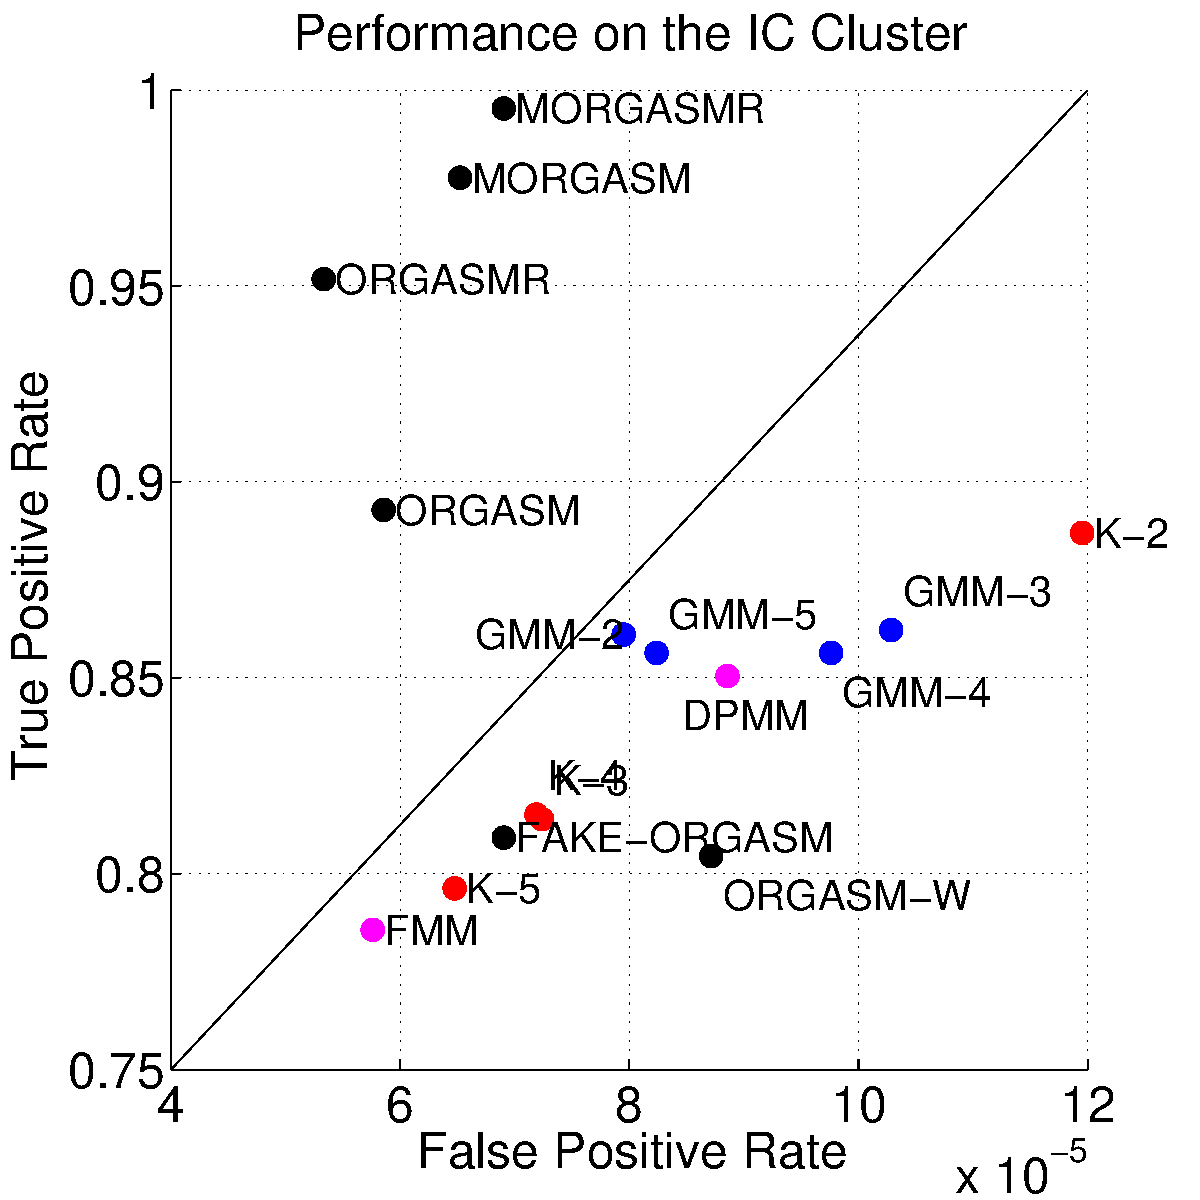
\includegraphics[width=\textwidth]{../figs/truefalsepositive.pdf}
\caption{}
\label{hc1res}
\end{subfigure}
\begin{subfigure}[b]{.49\textwidth}
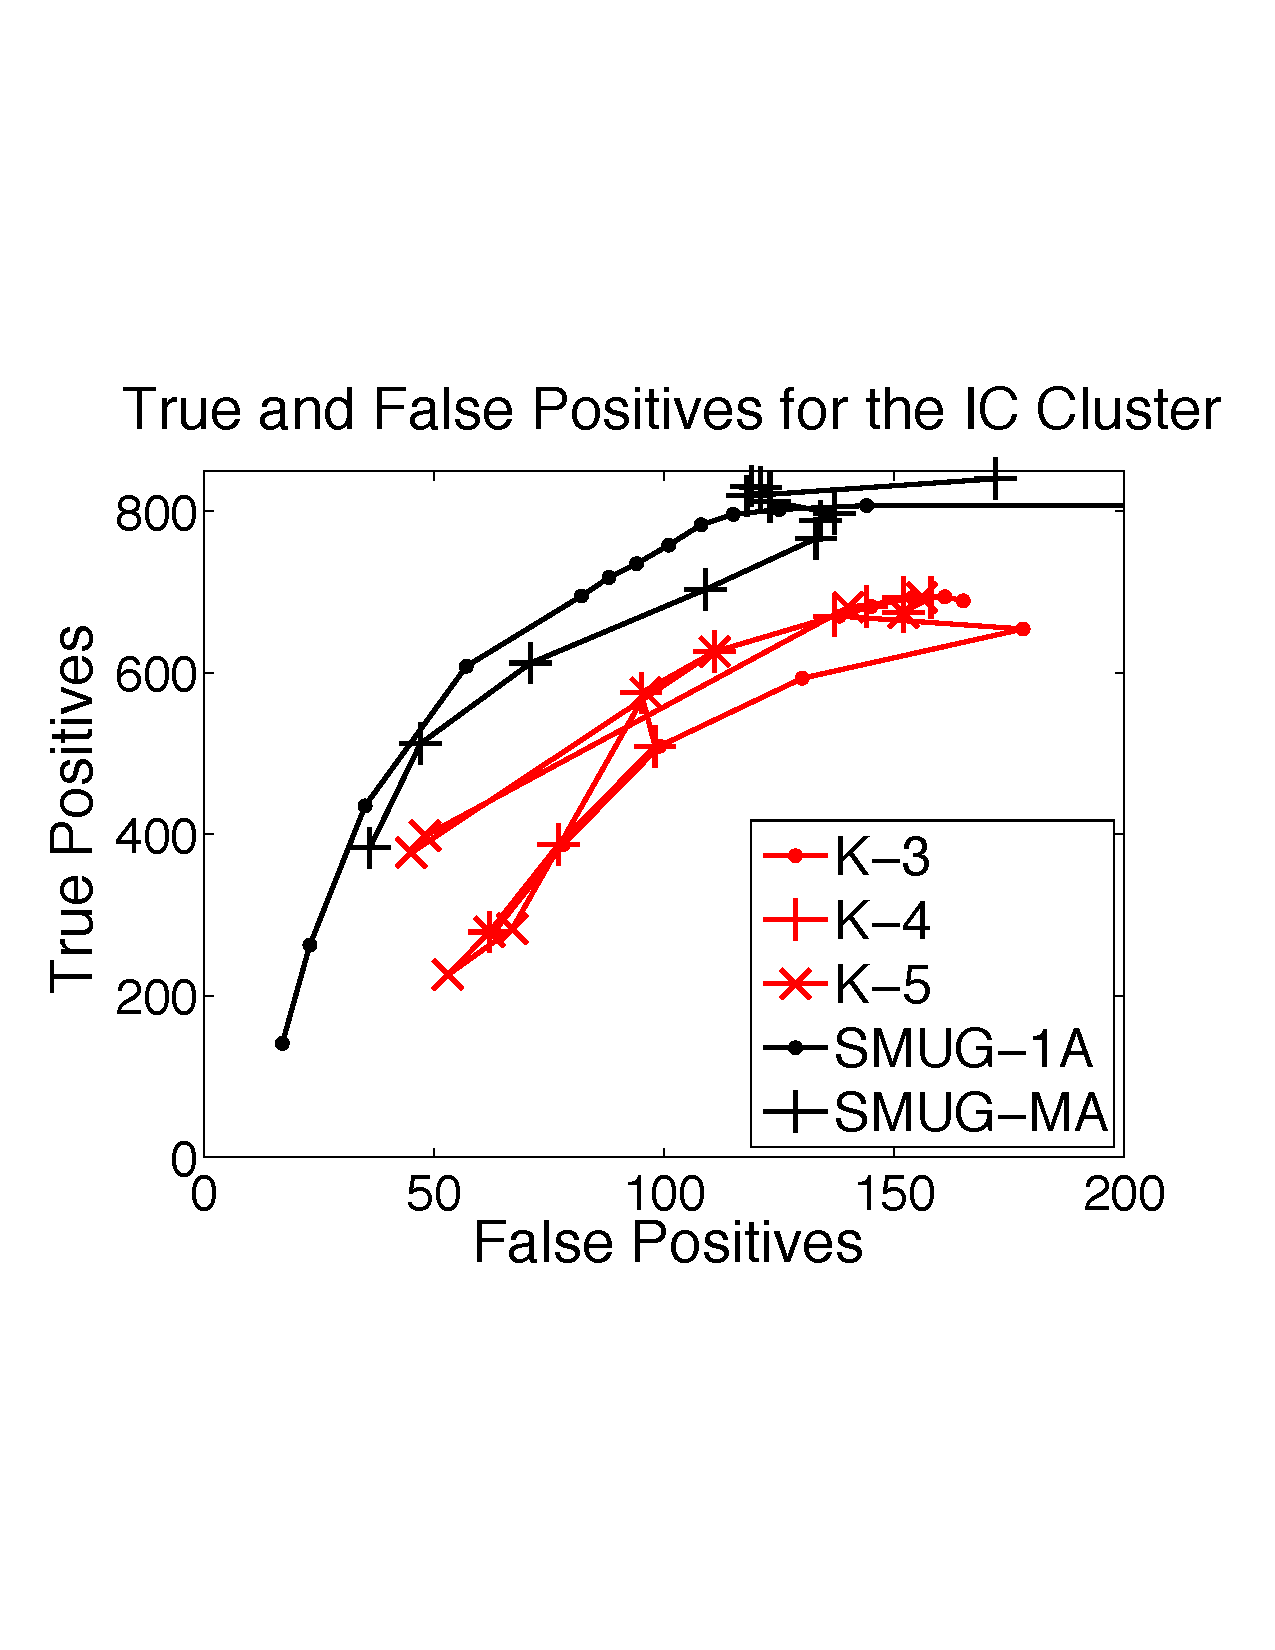
\includegraphics[width=\textwidth]{../figs/new/icroc.pdf}
\caption{}
\label{fig:roc}
\end{subfigure}
\caption{\smug\ achieves improved sensitivity and specificity over all competing methods on partial ground truth data (where true positives from one neuron are known from intracellular recordings).  
(a) True positive and false positive rates for all variants of \smug\ and several competing state-of-the-art \emph{batch} algorithms.  
(b) ROC curves demonstrating that both \sct{M}\smug\ and \smug\ outperform all competitor batch algorithms, regardless of threshold (including when we learn $\Lambda$ from the data, as indicated by a \jovo{*}).
\jovo{@dec - keep colors/symbols the same in the two panel, if possible.  maybe use a scheme where color indicates algorithm and shape indicates \# of components.  also, be consistent about "IC" cluster vs. "Intracellular" Cluster. and normalize, renaming axes XY Rate instead of only XY. (b) title should be ``ROC Curve Comparisons''}  
}
\end{figure}
\end{center}



\subsection{Overlapping Spike Detection}



A putative reason for the improved sensitivity and specificity of \smug\ over other algorithms is its ability to detect overlapping spikes.   When spikes overlap, although the result can accurately be modeled as a linear sum in voltage space, the resulting waveform often does not appear in any cluster in PC space (see \ref{Pillow2013}).  However, our online approach can readily find such overlapping spikes.  Figure \ref{fig:overlapping} shows one example of 135 examples where \smug\ believed that multiple waveforms were overlapping.  Indeed, it should be clear that by virtue of estimating the presence of multiple spikes, the residual squared error between the expected voltage and observed voltage shrinks.  Figure \ref{fig:resid} shows the density of the residual errors for all putative overlapping spikes.  The mass of this density is significantly smaller than the mass of the other scenarios.  Of all the true spikes that we detect, 37 of them we believe to be overlapping.  Thus, while it seems detecting overlapping spikes helps, it does not fully explain the improvements over the competitor algorithms.
\jovo{@jovo - add an actual statistical test test.} 


% It is possible for action potentials to fire close to simultaneously so that a given window would have 2 or move action potent ions.  It is possible for the algorithm to detect and fit overlapping spikes as they come in.  Out of the 3593 spikes detected by the algorithm, there are 124 pairs of overlapping spikes within 1 ms of one another (3.45\%).  An example of an overlapping waveform is shown in Figure \ref{overlapping}.


\begin{center}
\begin{figure}[h!]
\begin{subfigure}[b]{.49\textwidth}
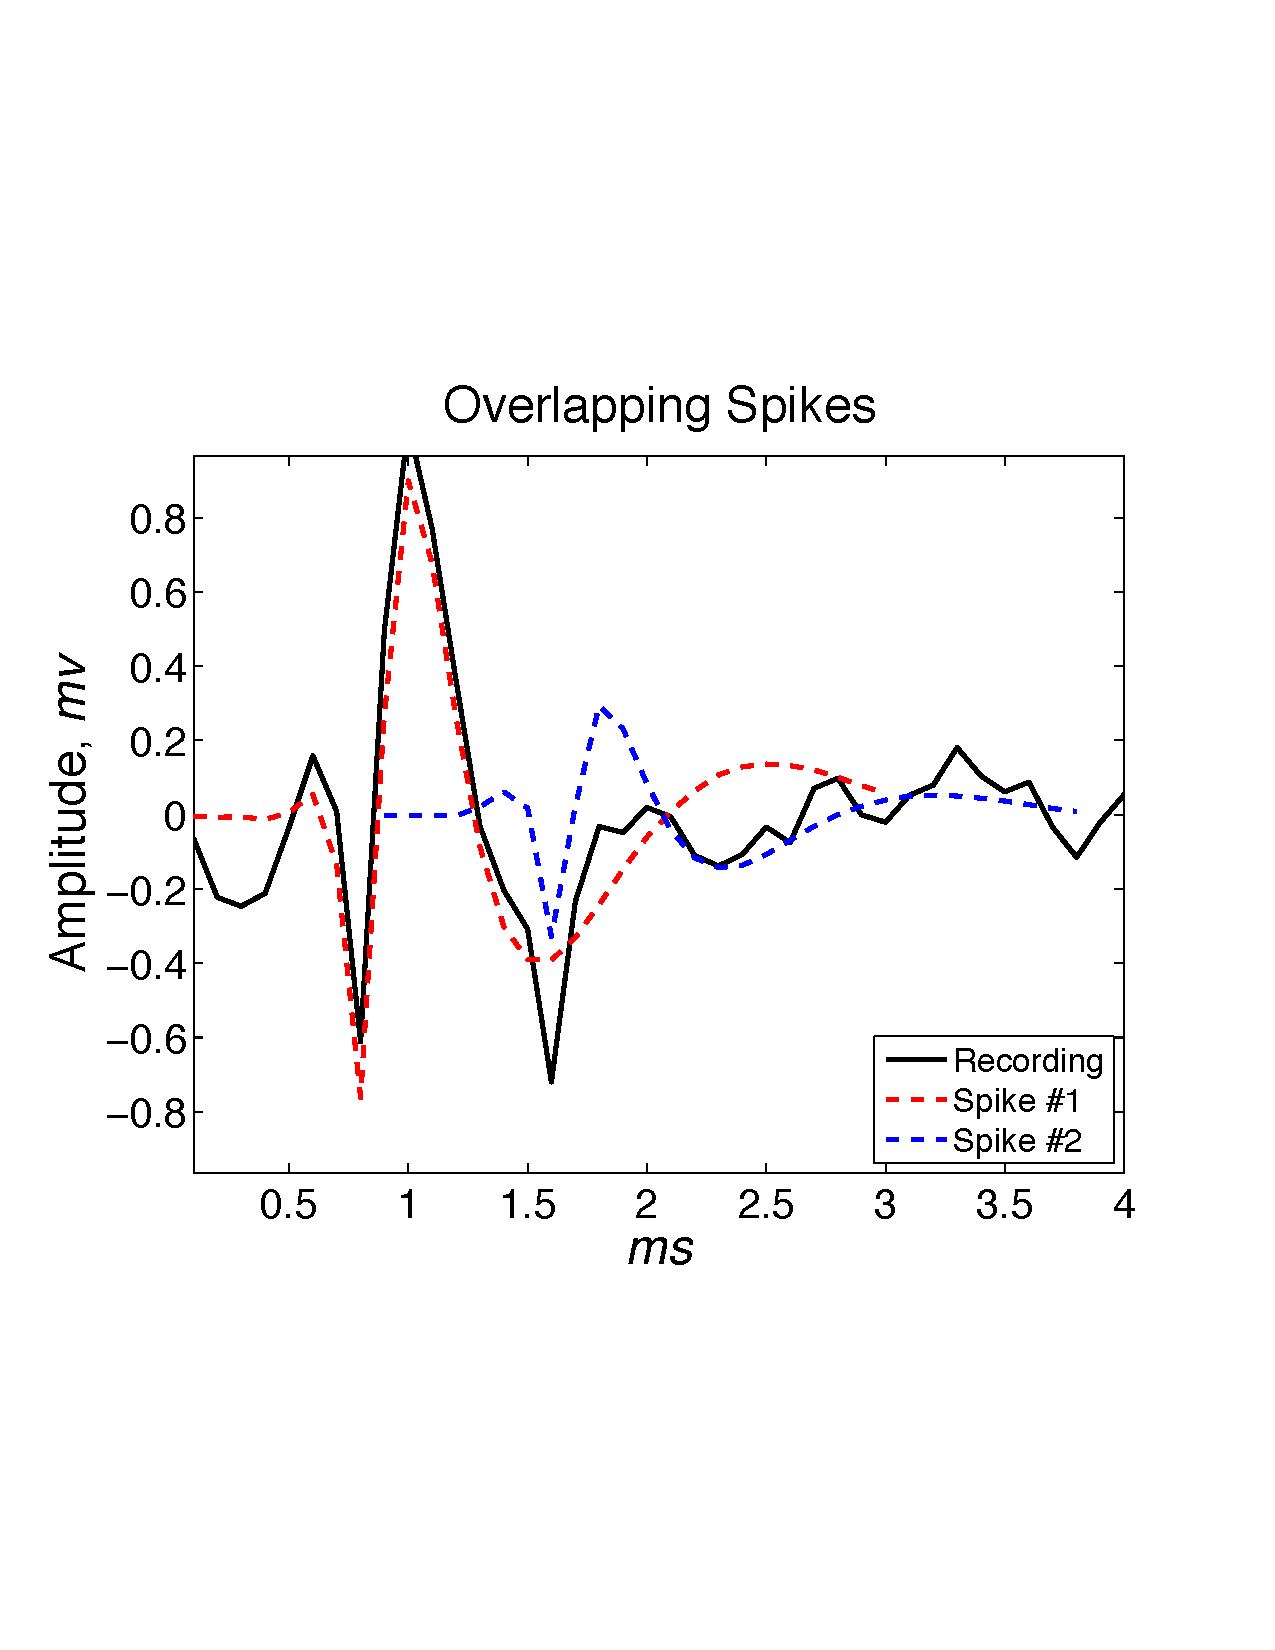
\includegraphics[width=\textwidth]{../figs/alloverlappingspikes/olspike3}
\caption{}
\label{fig:overlapping}
\end{subfigure}
\begin{subfigure}[b]{.49\textwidth}
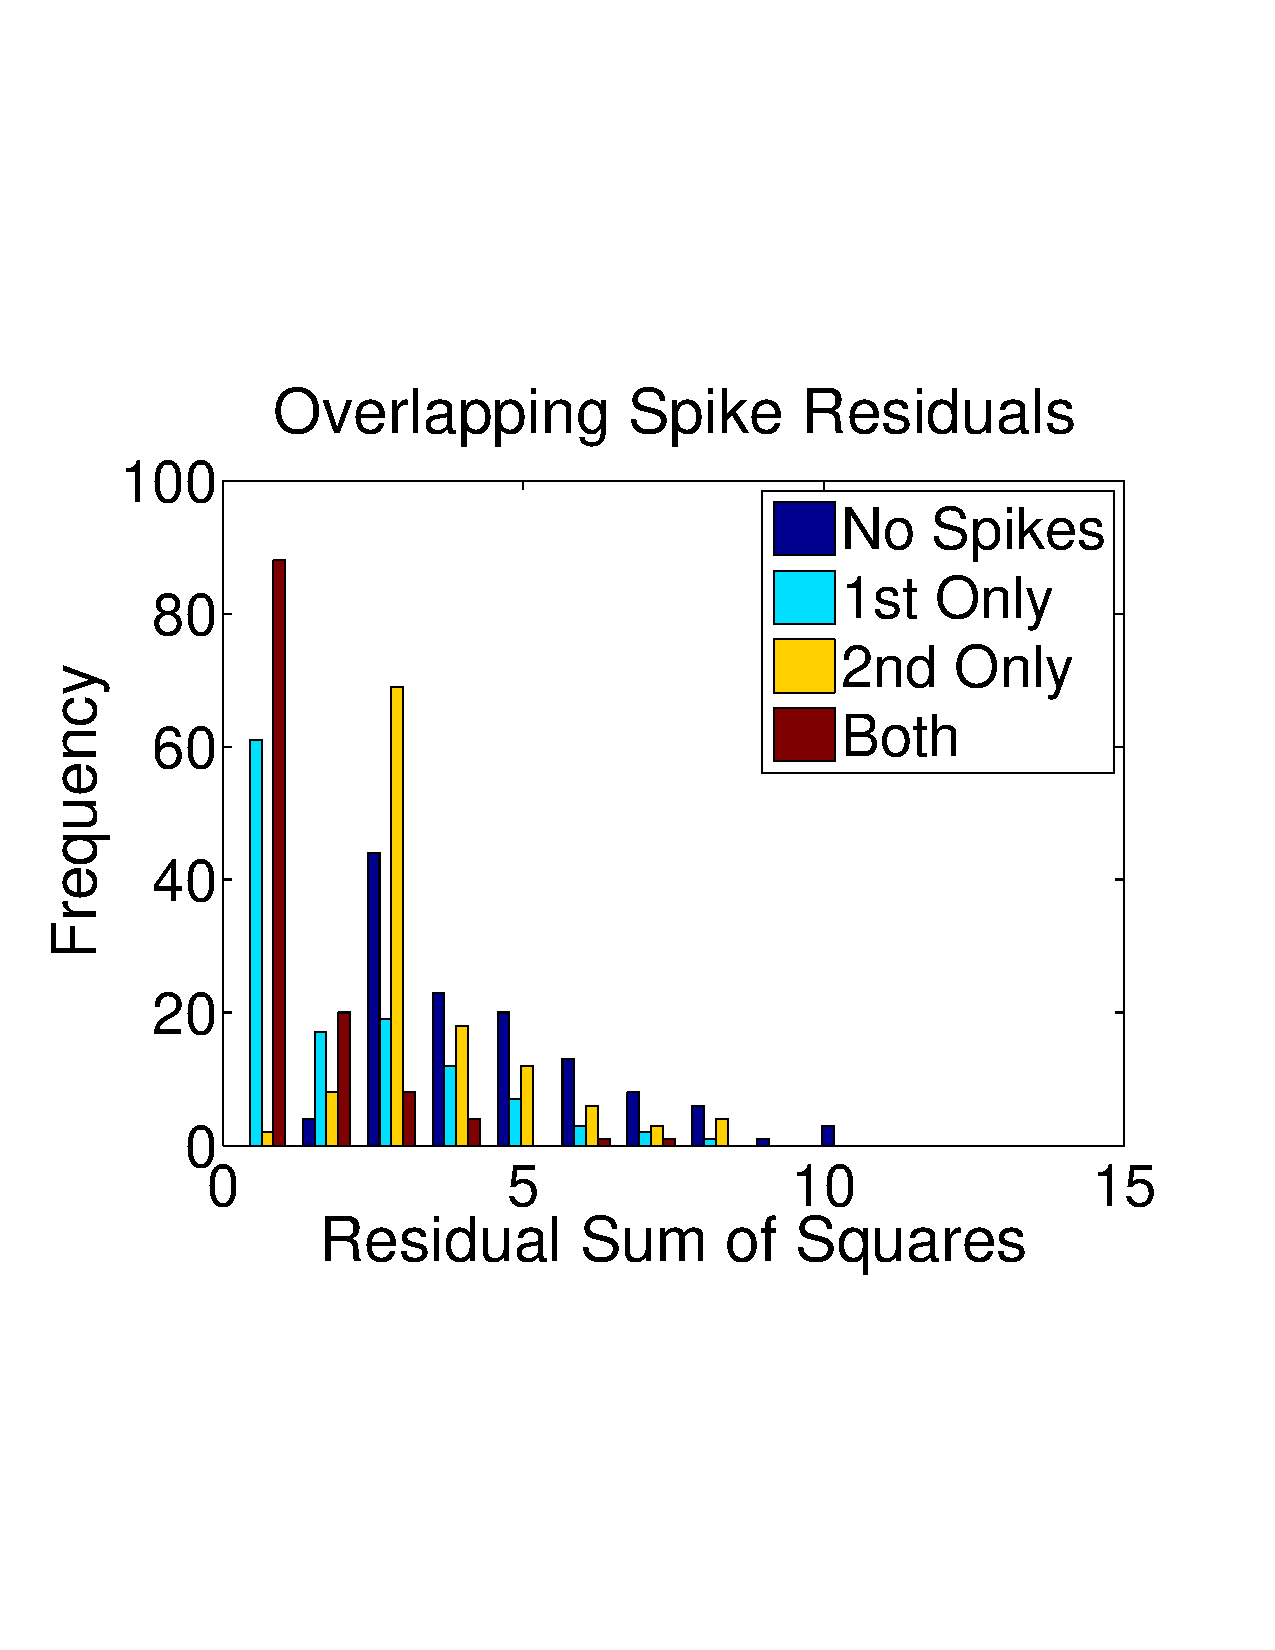
\includegraphics[width=\textwidth]{../figs/overlappingstat.pdf}
\caption{}
\label{fig:resid}
\end{subfigure}
\caption{Results on the d533101 dataset.  (a) \jovo{like this but also with the sum} (b) \jovo{residuals for this example.} (c) \jovo{histogram of residuals for all putative overlapping examples. keep colors consistent across all three panels.  i think line plots for the histograms would more clearly indicate that residuals are significantly smaller than the others.}}
\end{figure}
\end{center}



\subsection{Time-Varying Waveform Adaptation} \label{sub:adapt}


As as been demonstrated previously \cite{calabrese2011kalman}, the waveform shape of a neuron may change over time.  The mean waveform over time for the intracellular neuron is shown in Figure \ref{evohc1}.  Allowing the mean of each component to evolve over time improved single-channel performance over the 4-minute dataset, and gave similar performance in the multi-channel algorithms.


\begin{center}
\begin{figure}
\begin{subfigure}[b]{.33\textwidth}
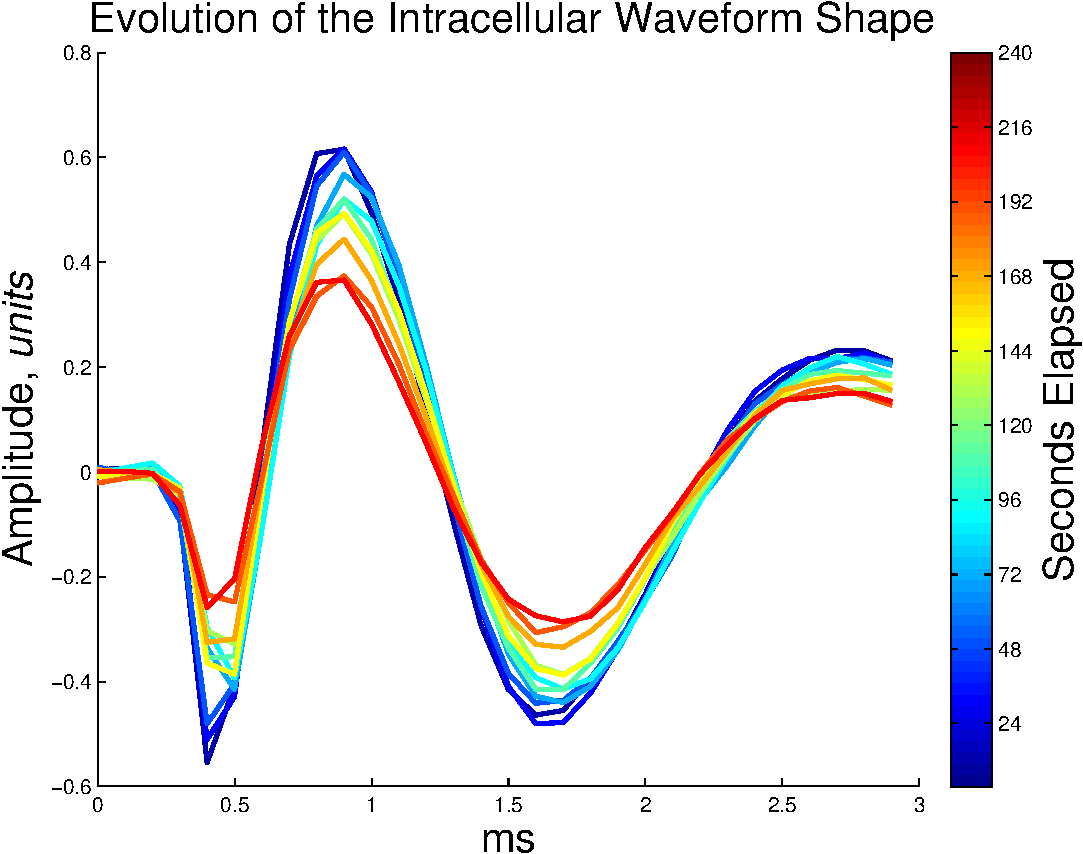
\includegraphics[width=\textwidth]{../figs/evohc1}
\caption{}
\label{evohc1}
\end{subfigure}
\begin{subfigure}[b]{.33\textwidth}
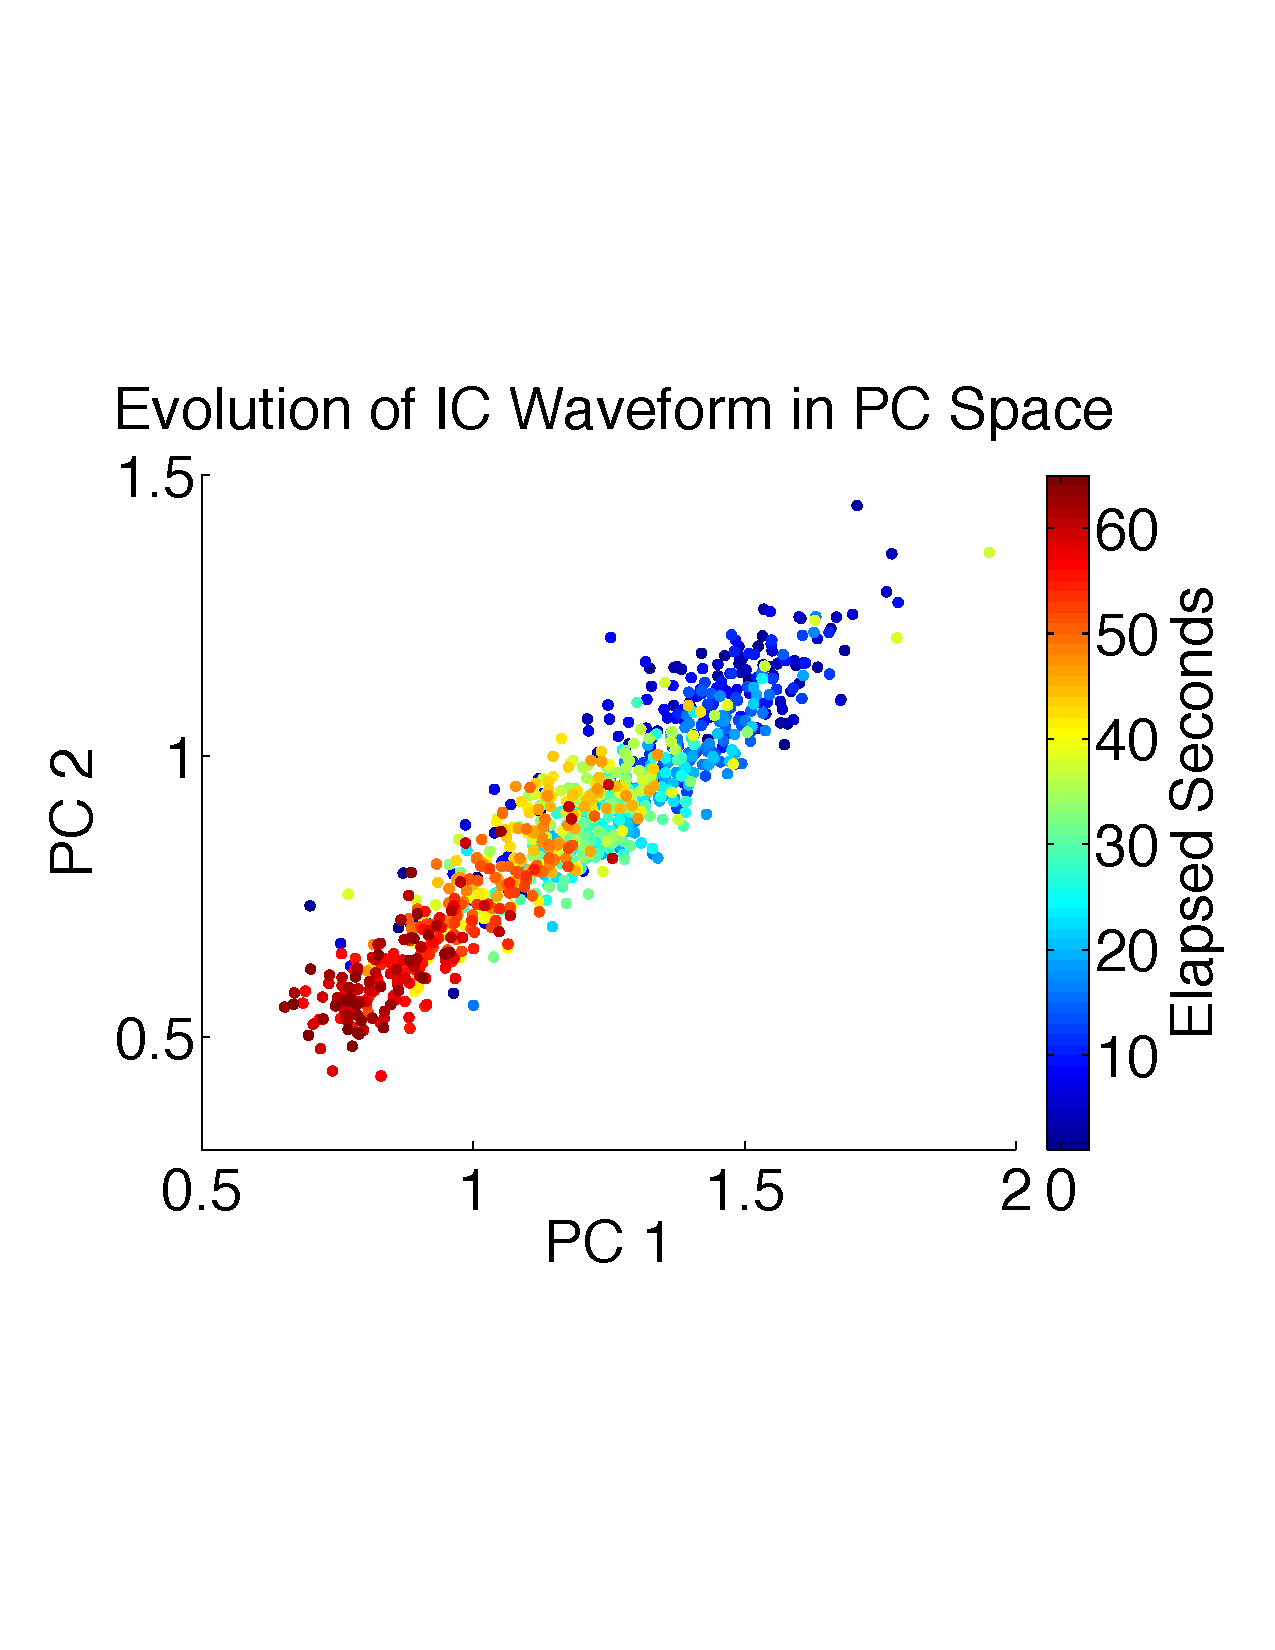
\includegraphics[width=\textwidth]{../figs/new/clusterevo.pdf}
\caption{}
\label{clusterevo}
\end{subfigure}
\begin{subfigure}[b]{.33\textwidth}
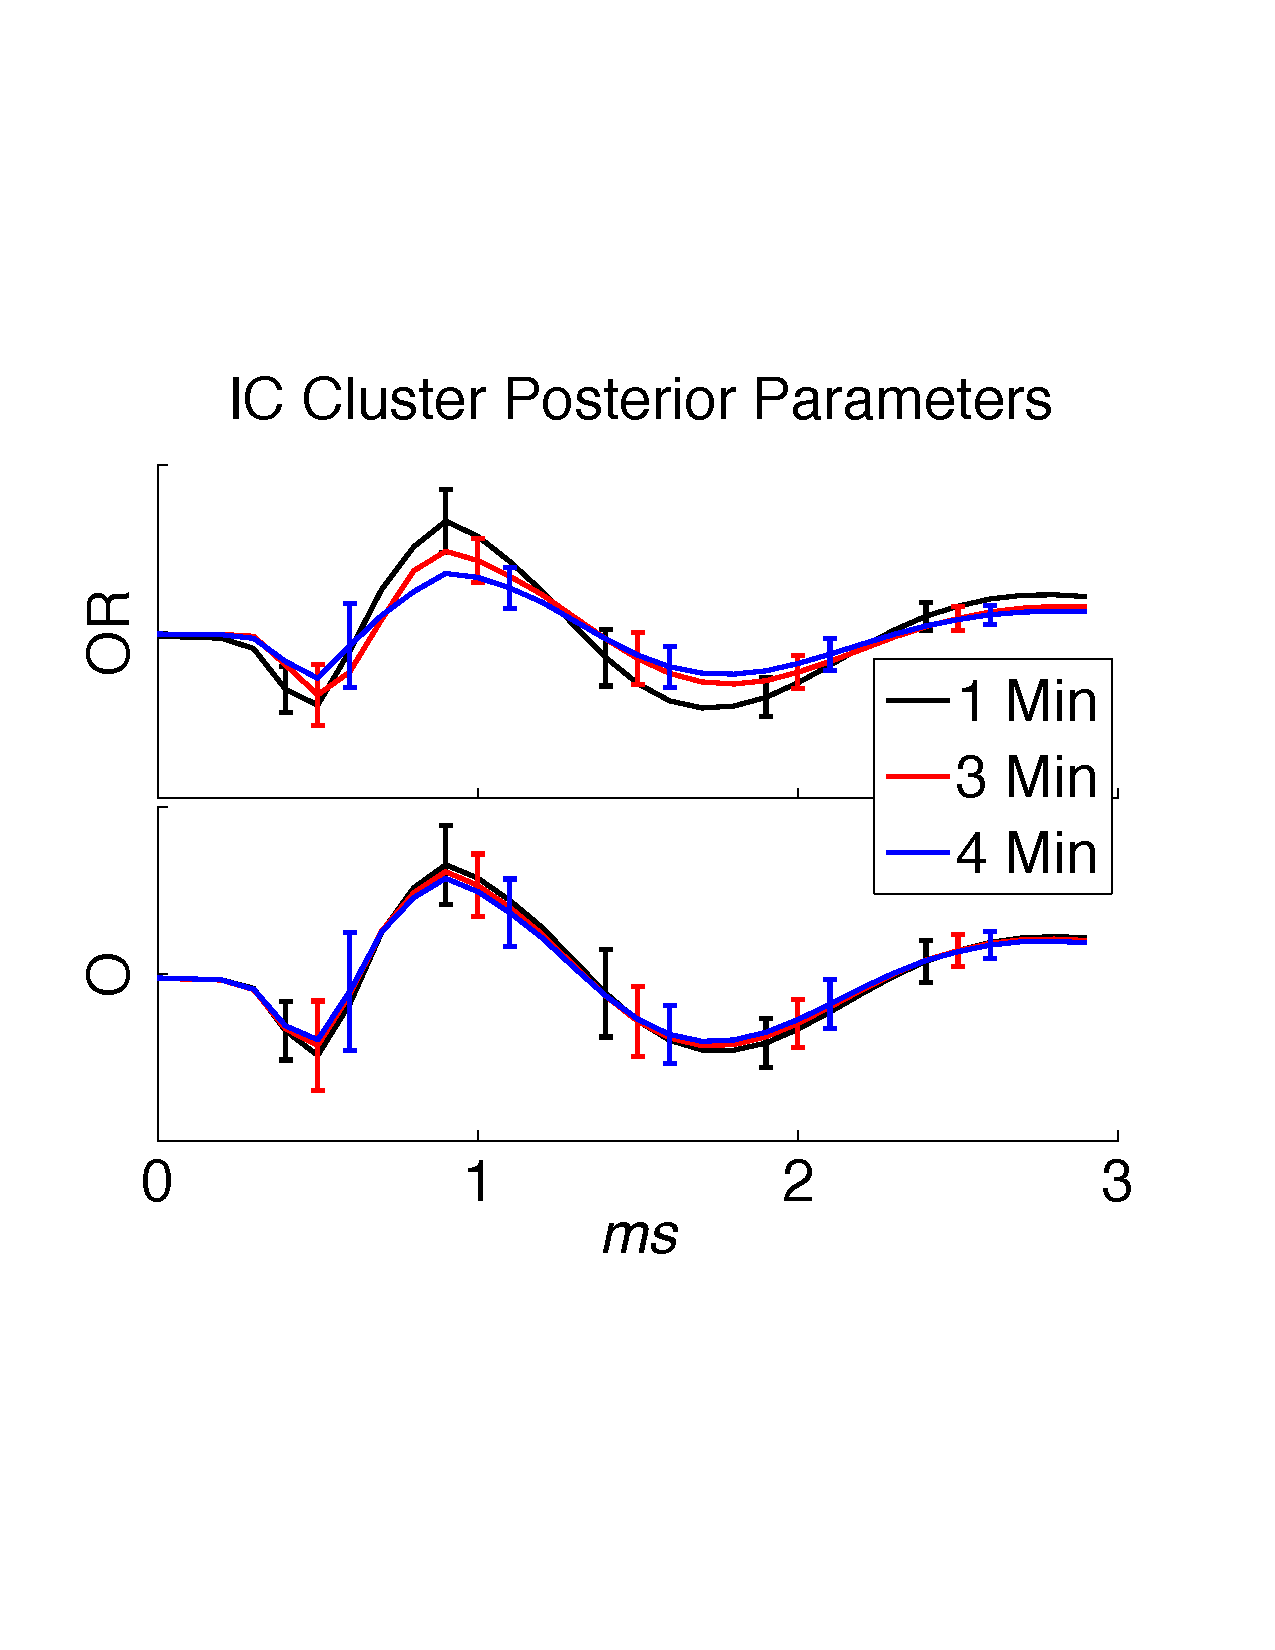
\includegraphics[width=\textwidth]{../figs/new/ARvsStationary.pdf}
\caption{}
\label{truewaveforms}
\end{subfigure}
\caption{
(a) Mean IC waveforms over time.  Each colored line represents the mean of the waveform averaged over 24s and the color gives the elapsed time.  This neuron decreases in amplitude over the period of the recording. 
(b) \jovo{take out scale bars.}
(c) \jovo{plot 3 ARs on top of each other, and also plot 3 stationary on top of each other.}}
\end{figure}
\end{center}

\subsection{Multi-Electrode Array} \label{sub:multi}

\jovo{add grids to all panels of all figs by default, remove if it looks shitty.}


In the tetrode case the waveform undoubtedly appears on all channels at once; it is possible to concatenate the channels to jointly process the data \cite{wood2009}.  When the action potential will only appear on a subset of channels it is nice to allow the action potential to vary in a low-dimensional subset in each of the channels instead of a low-dimensional subset over all the channels. \cite{Prentice2011}

We use processed data from novel NeuroNexus devices implanted in the rat motor cortex.  The data was recorded at 32.5kHz in freely-moving rats, and the data was first processed by high-pass filtering at 800Hz.  The first device we consider is a set of 3 channels of data shown in Figure \ref{3dev}.  The neighboring electrode sites in these devices have 30 $\mu$m between electrode edges and 60 $\mu$m between electrode centers.  These devices are close enough that a locally-firing neuron could appear on multiple electrode sites (cite that paper on action potential overlap), and neighboring channels warrant joint processing.  The second, 8-channel device is shown in Figure \ref{8dev}, and has similar properties to the first device.

 The top 2 clusters found in the first 10 minutes of data on the 3-channel device are shown in Figures \ref{ex31}, \ref{ex32}.  The waveform in channel 3 is very similar for the waveforms in Figure \ref{ex31} and \ref{ex32}, and would be difficult to separate if we were analyzing each channel individually; the representation of those two clusters in PCA space on channel 3 is shown in Figure \ref{chpca}.  We gain the ability to distinguish the waveforms by looking at all the channels simultaneously.  The top 3 clusters found in the 8-channel device can be found in Figures \ref{ex81}, \ref{ex82}, and \ref{ex83}.

{\color{red} perhaps add comments about time-evolution and the false positives we avoid by using multi-channel analysis}


\begin{center}
\begin{figure}
\begin{subfigure}[b]{.12\textwidth}
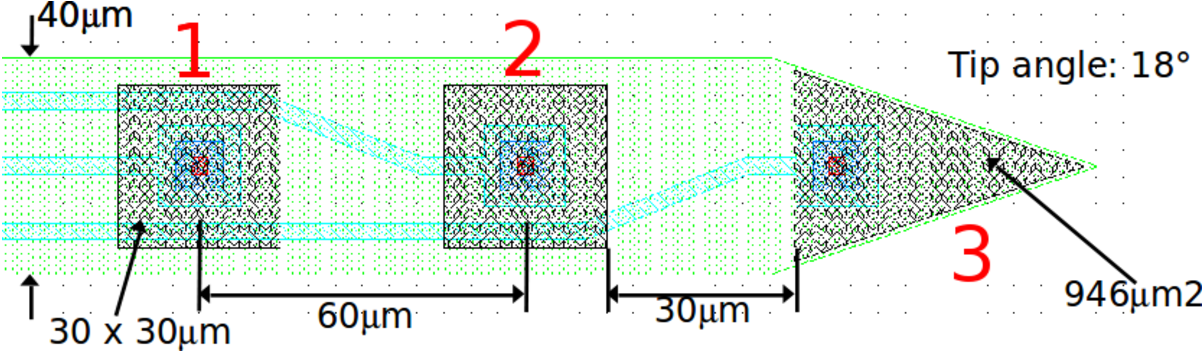
\includegraphics[width=1\textwidth]{../figs/3dev}
\caption{}
\label{3dev}
\end{subfigure}
\begin{subfigure}[b]{.28\textwidth}
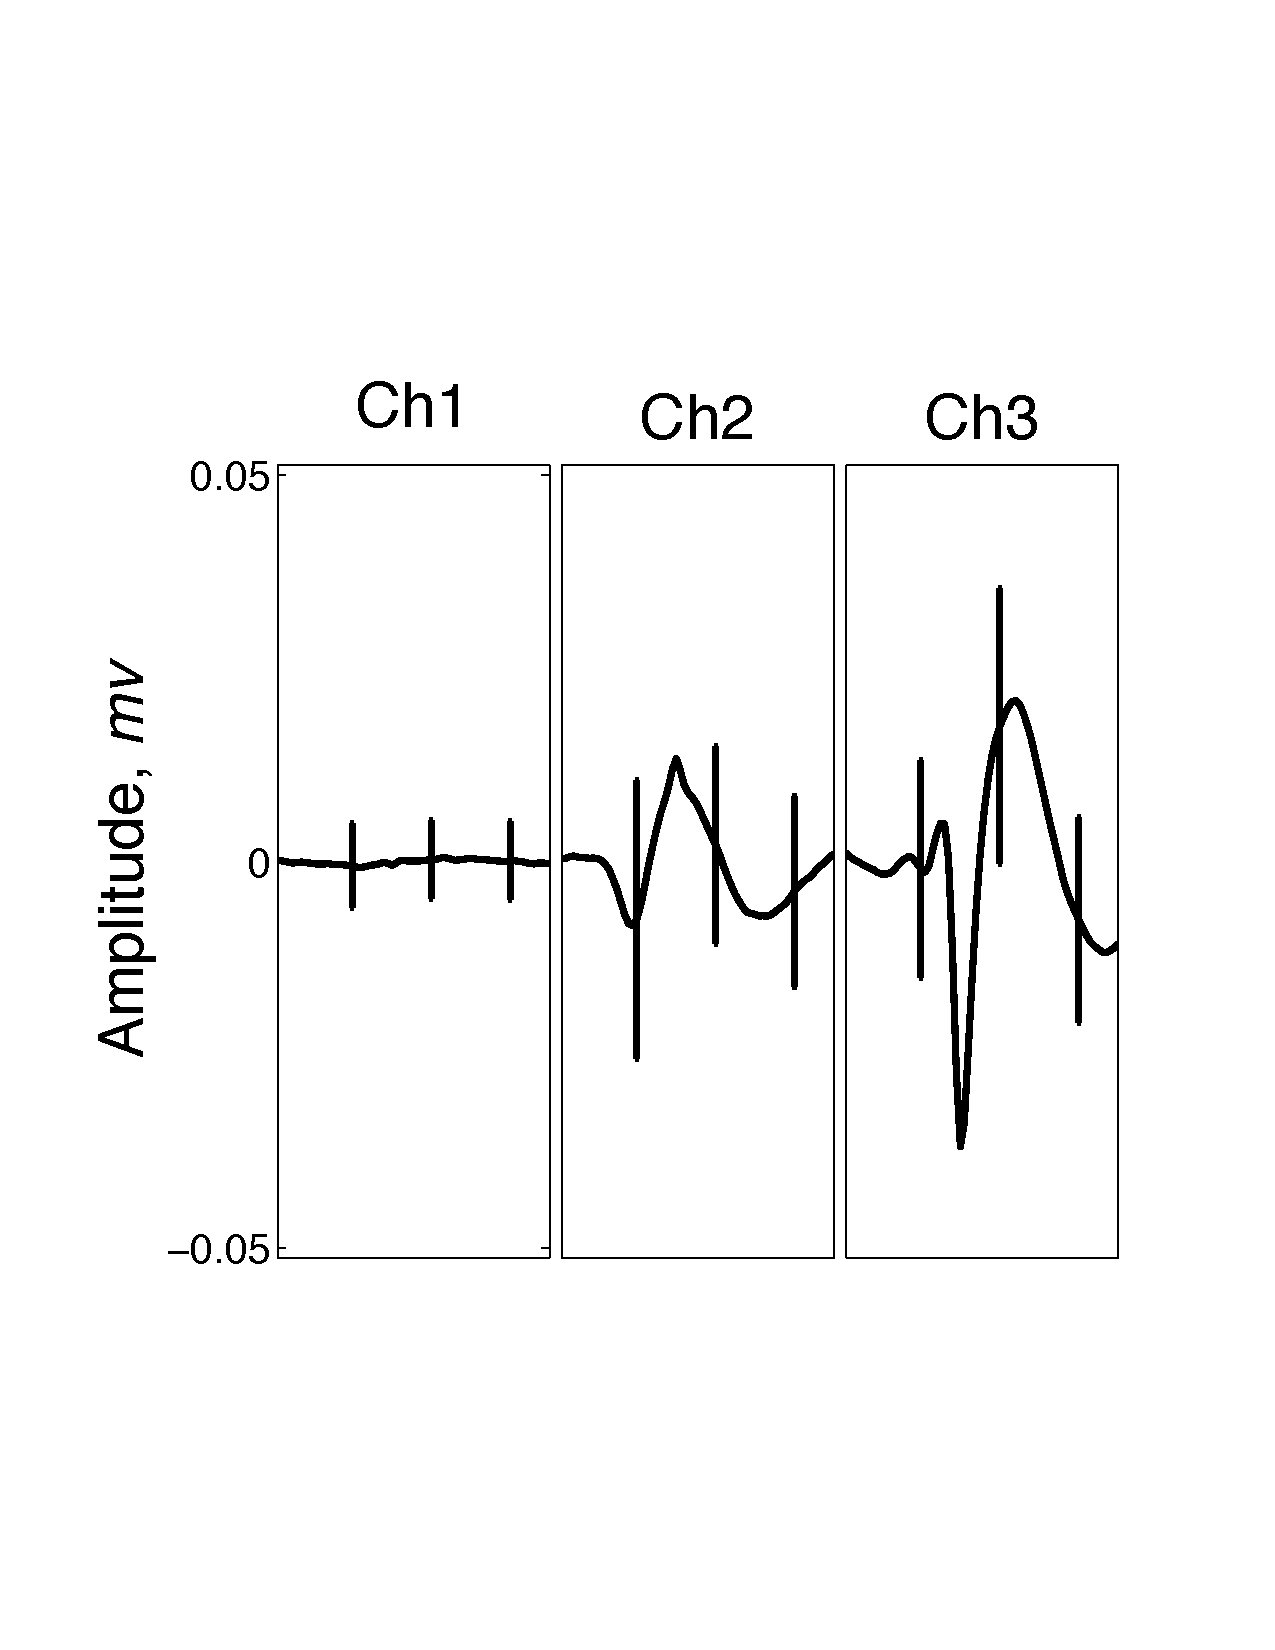
\includegraphics[width=\textwidth]{../figs/3devim/clus1}
\caption{}
\label{ex31}
\end{subfigure}
\begin{subfigure}[b]{.28\textwidth}
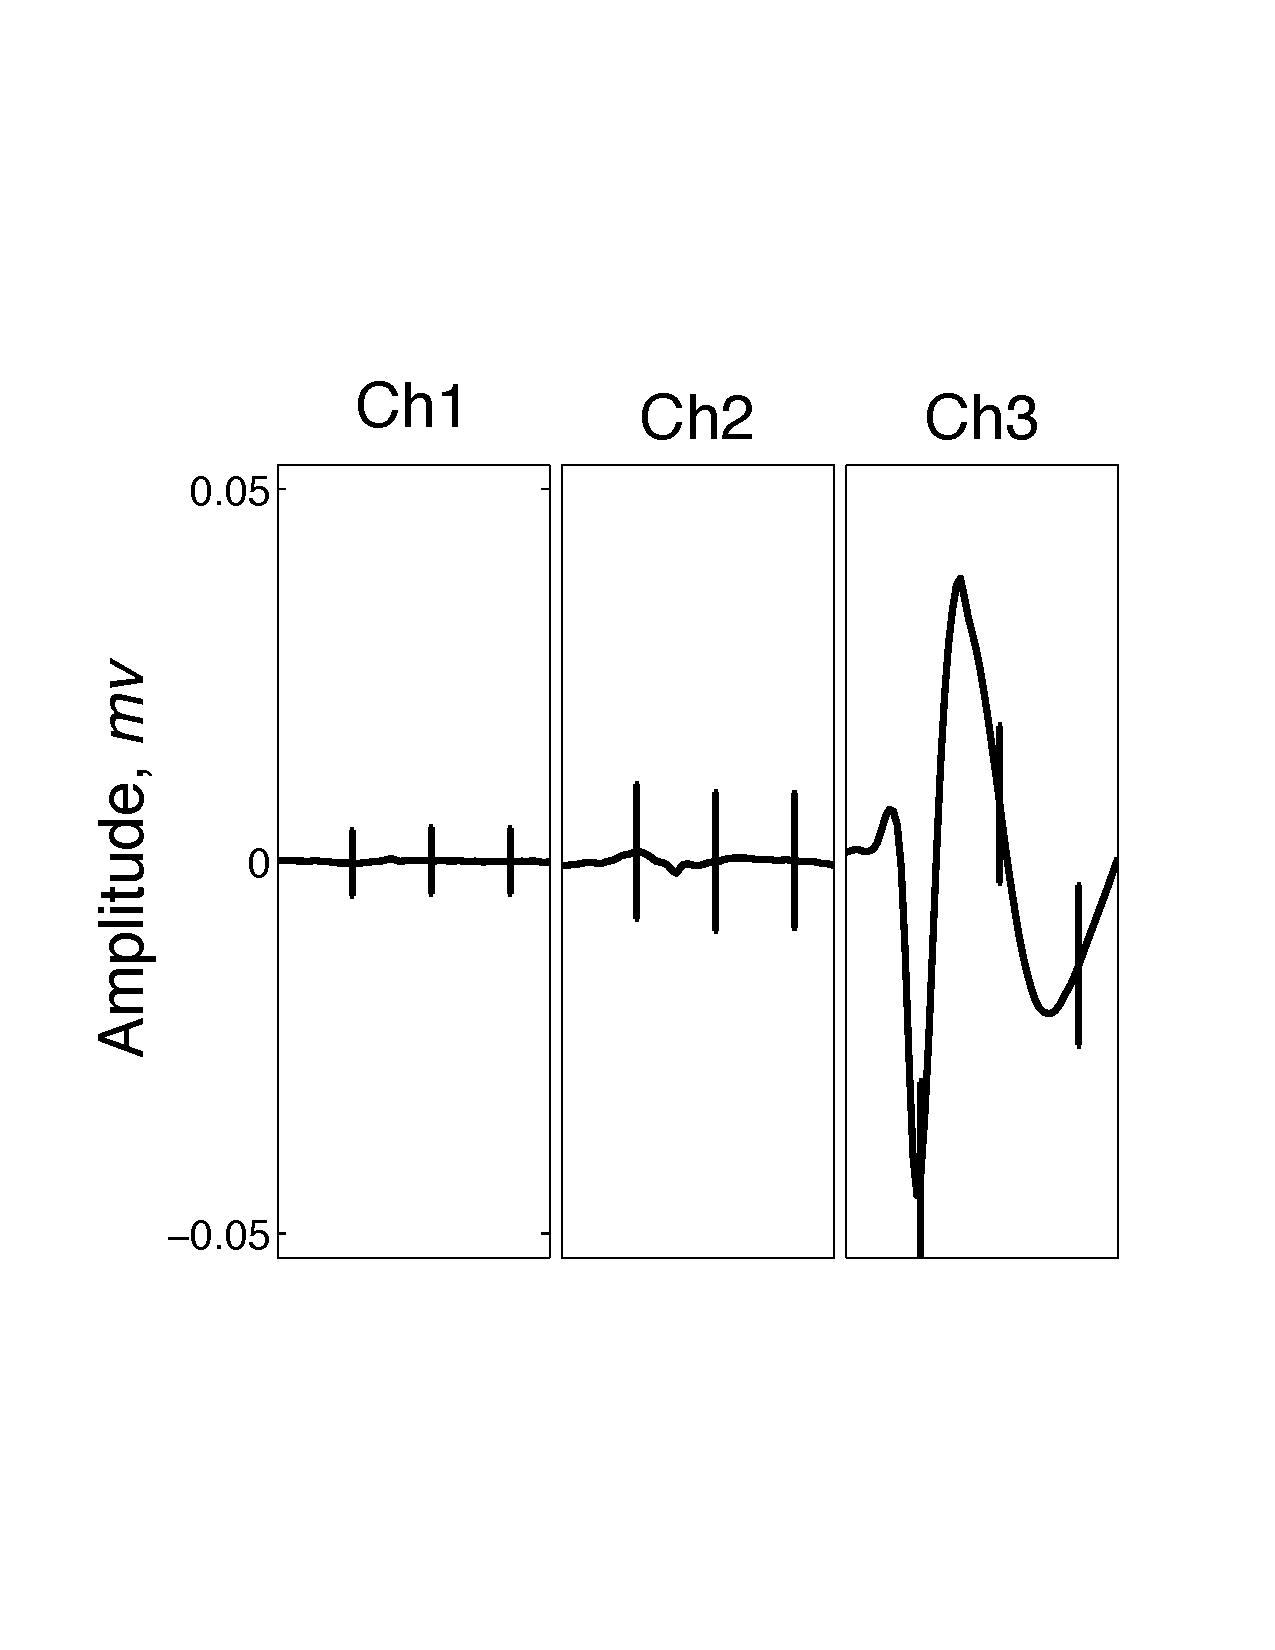
\includegraphics[width=\textwidth]{../figs/3devim/clus2}
\caption{}
\label{ex32}
\end{subfigure}
\begin{subfigure}[b]{.28\textwidth}
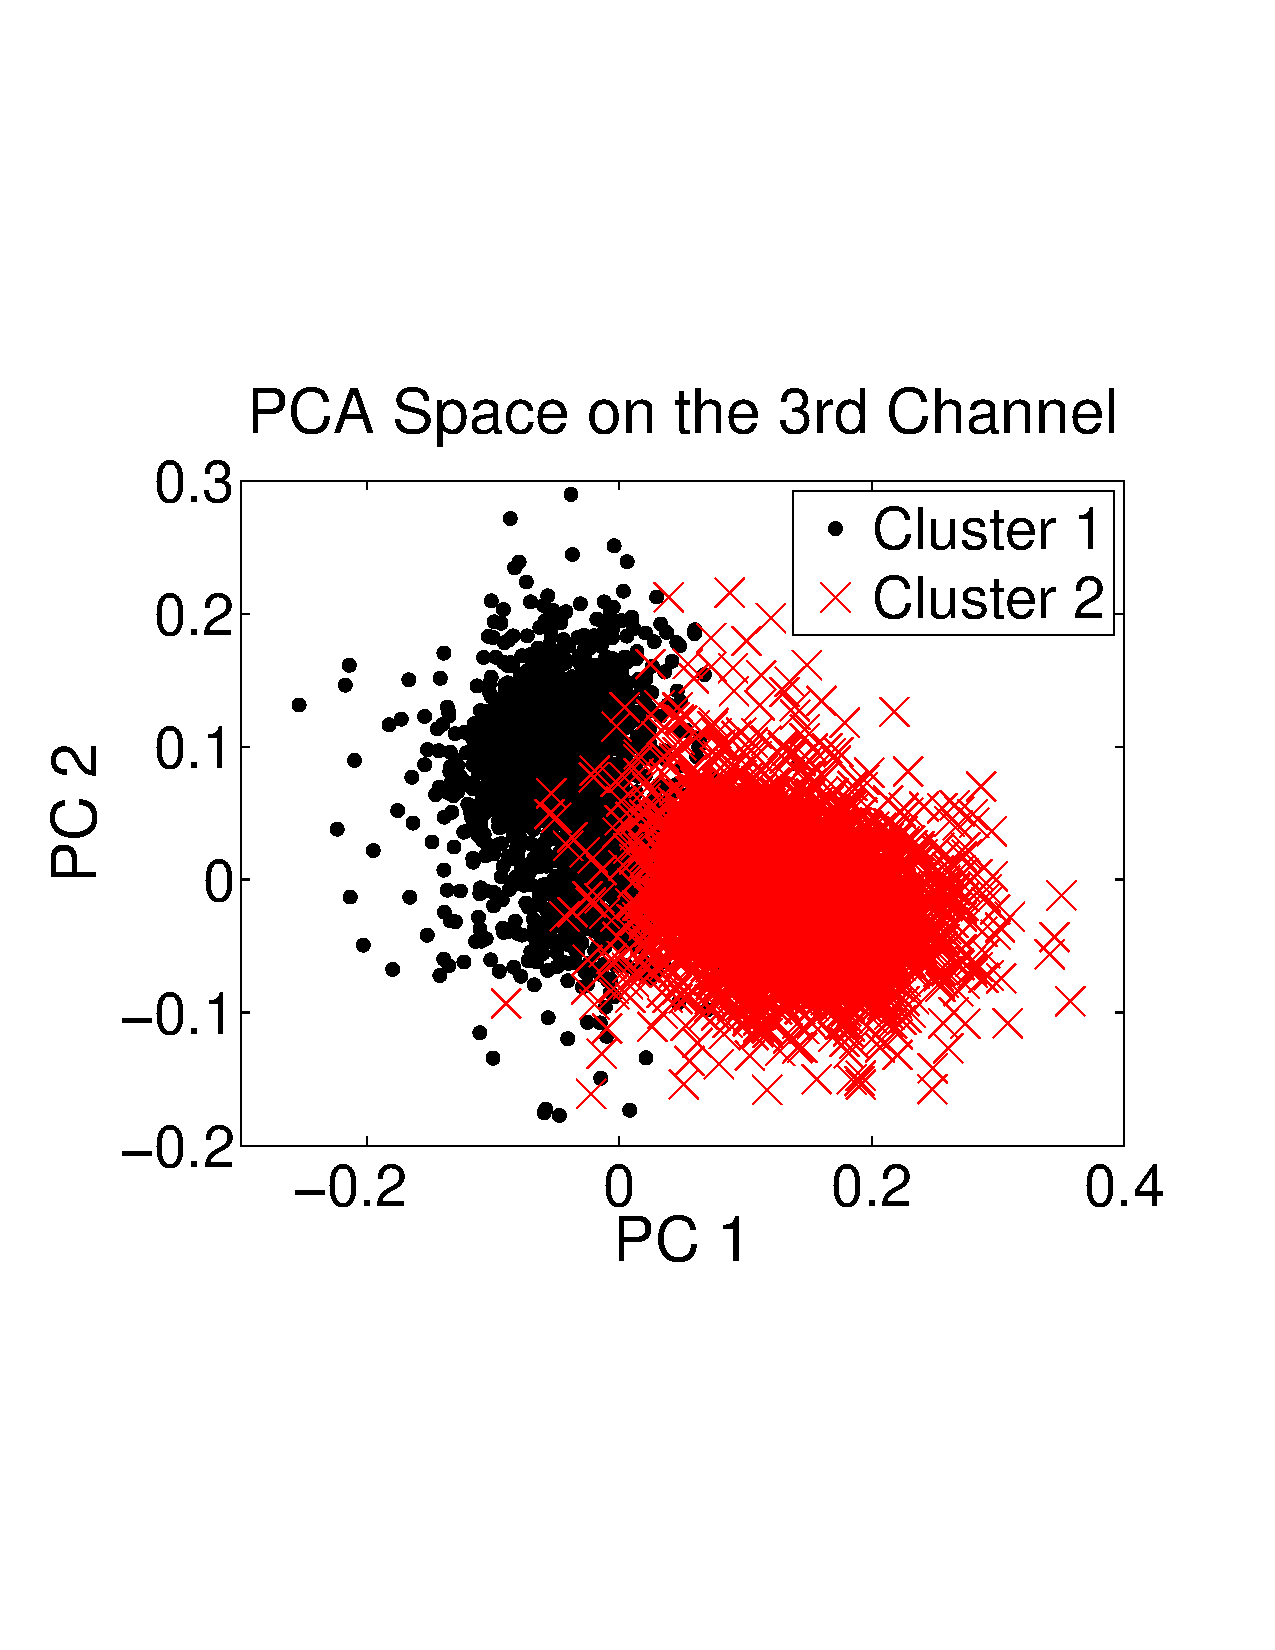
\includegraphics[width=\textwidth]{../figs/new/3chpca}
\caption{}
\label{3chpca}
\end{subfigure}
% \caption{}
% \end{figure}
% \end{center}
% \begin{center}
% \begin{figure}[h!]
\begin{subfigure}[b]{.12\textwidth}
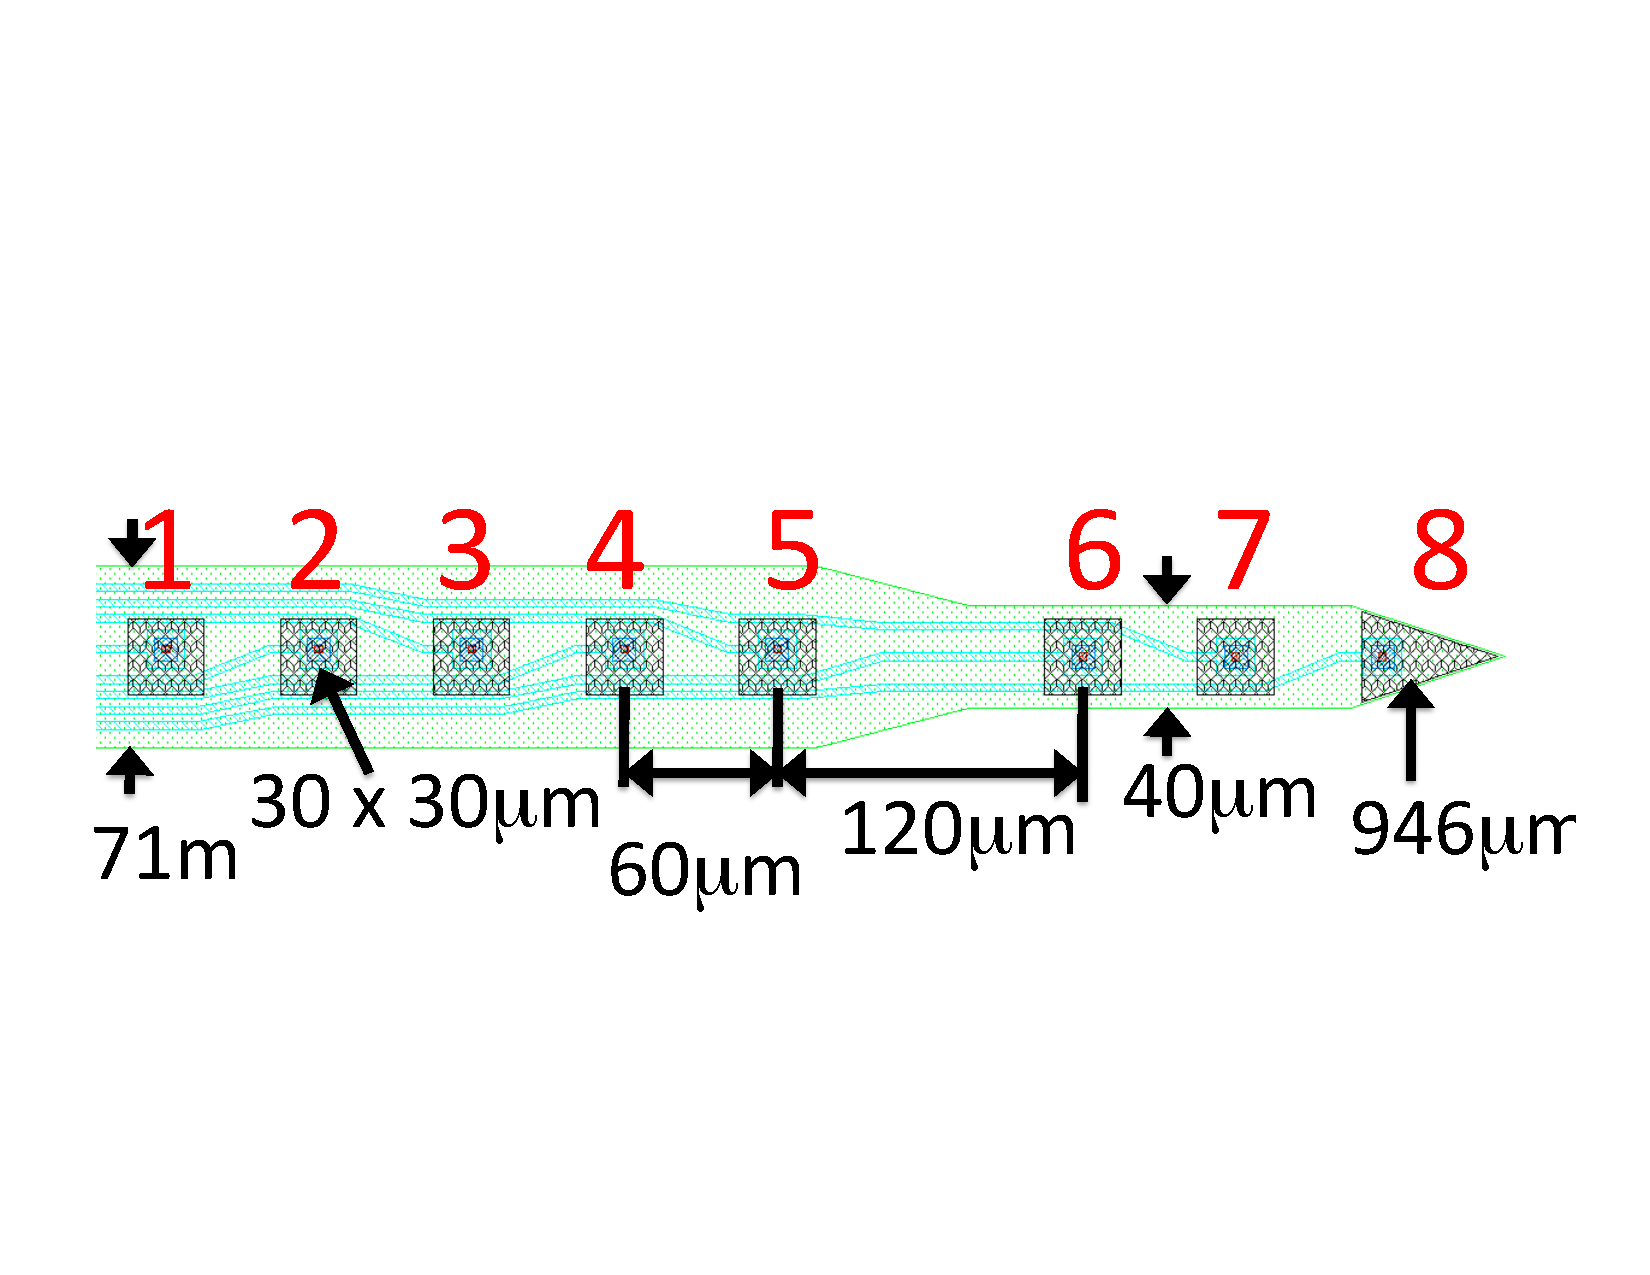
\includegraphics[width=0.8\textwidth]{../figs/8dev}
\caption{}
\label{3dev}
\end{subfigure}
\begin{subfigure}[b]{.28\textwidth}
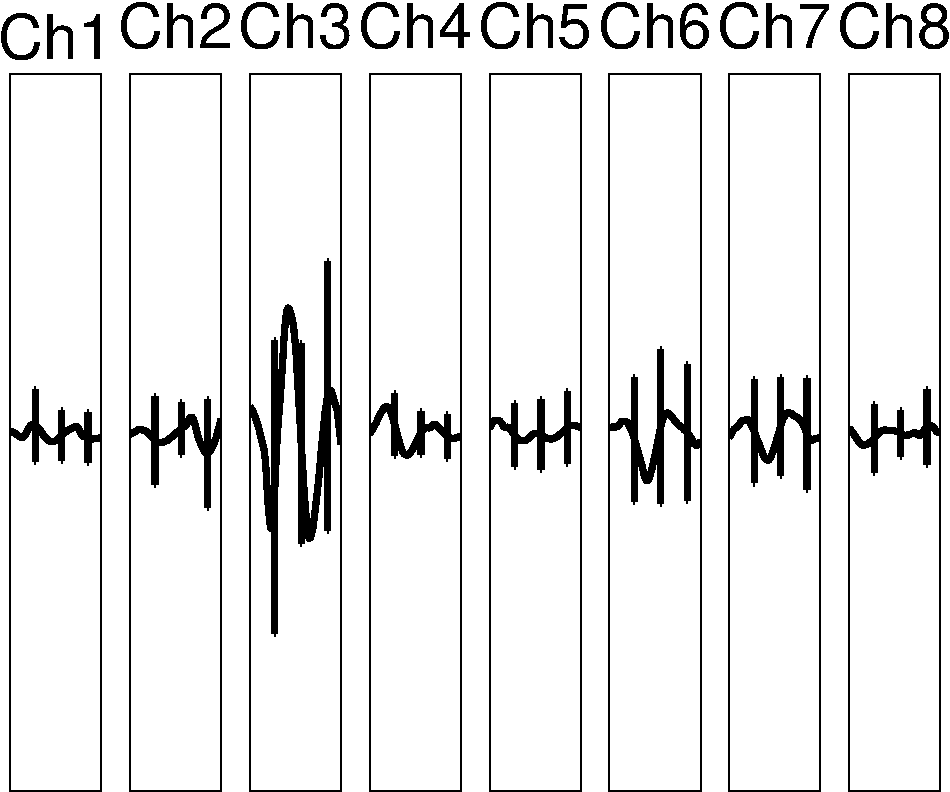
\includegraphics[width=\textwidth]{../figs/8devim/clus3}
\caption{}
\label{ex81}
\end{subfigure}
\begin{subfigure}[b]{.28\textwidth}
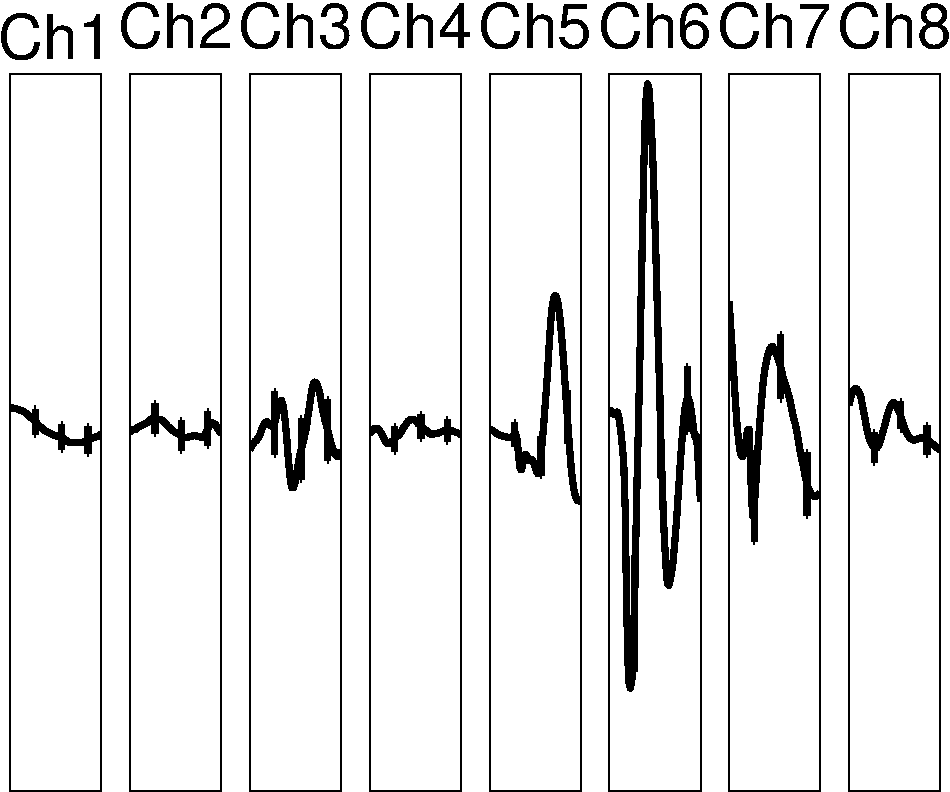
\includegraphics[width=\textwidth]{../figs/8devim/clus9}
\caption{}
\label{ex82}
\end{subfigure}
\begin{subfigure}[b]{.28\textwidth}
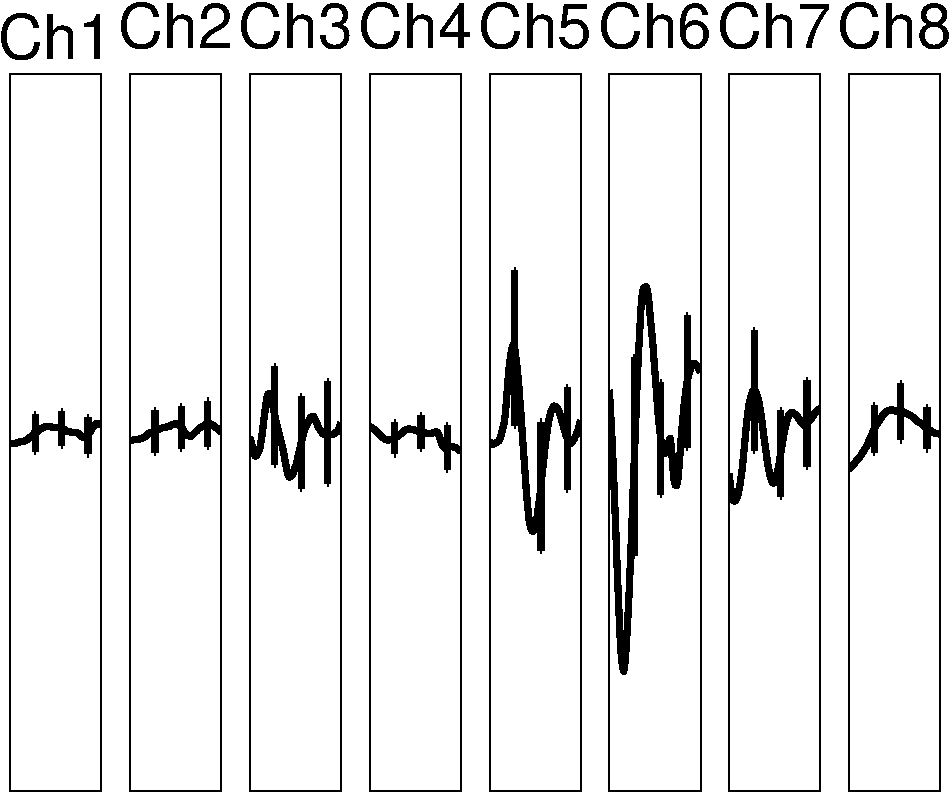
\includegraphics[width=\textwidth]{../figs/8devim/clus6}
\caption{}
\label{ex83}
\end{subfigure}
\caption{
(a) Three electrode device showing local proximity of electrodes with channel indexes in large, red numbers. (b,c) Top 2 most prevalent waveforms.  Each waveform shape is 2ms long.   Note in (a) we have a waveform that appears on both channel 2 and channel 3, whereas in (b) the waveform only appears in channel 3.  If only channel 3 was used, it would be difficult to separate the waveform in (a) and (b), as is demonstrated in Figure (d) by the representation of detected spikes on the 3rd channel in PCA space.
(e)8 electrode device showing local proximity of electrodes with channel indexes in large, red numbers. (f,g,h) Top 3 most prevalent waveforms.  Each waveform shape is 2ms long.
\jovo{update these in various ways that you know.}
}
\end{figure}
\end{center}




\subsection{Limitations of Dictionary-Based Techniques} \label{sub:template}



\begin{center}
\begin{figure}[h!]
\begin{subfigure}[b]{.33\textwidth}
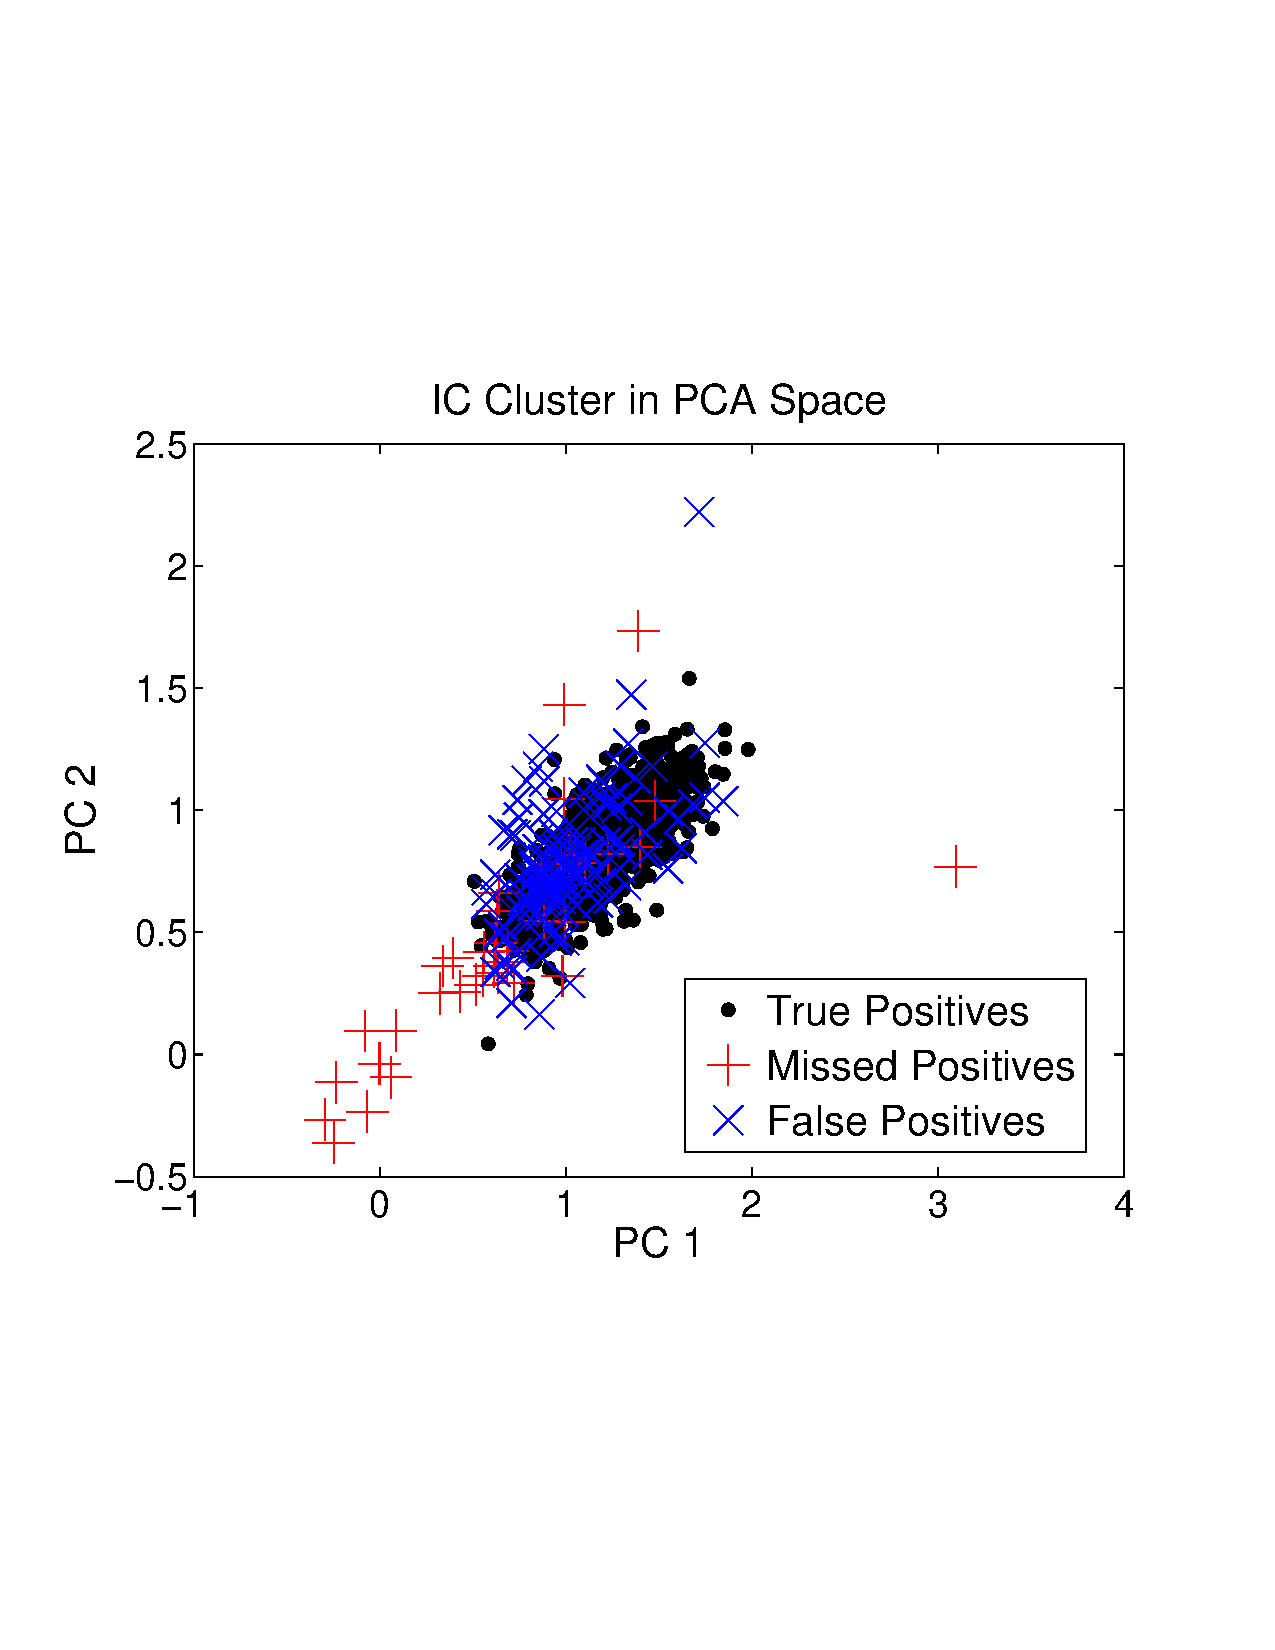
\includegraphics[width=\textwidth]{../figs/new/ICclusteroldpca.pdf}
\caption{}
\label{fig:ICold}
\end{subfigure}
\begin{subfigure}[b]{.33\textwidth}
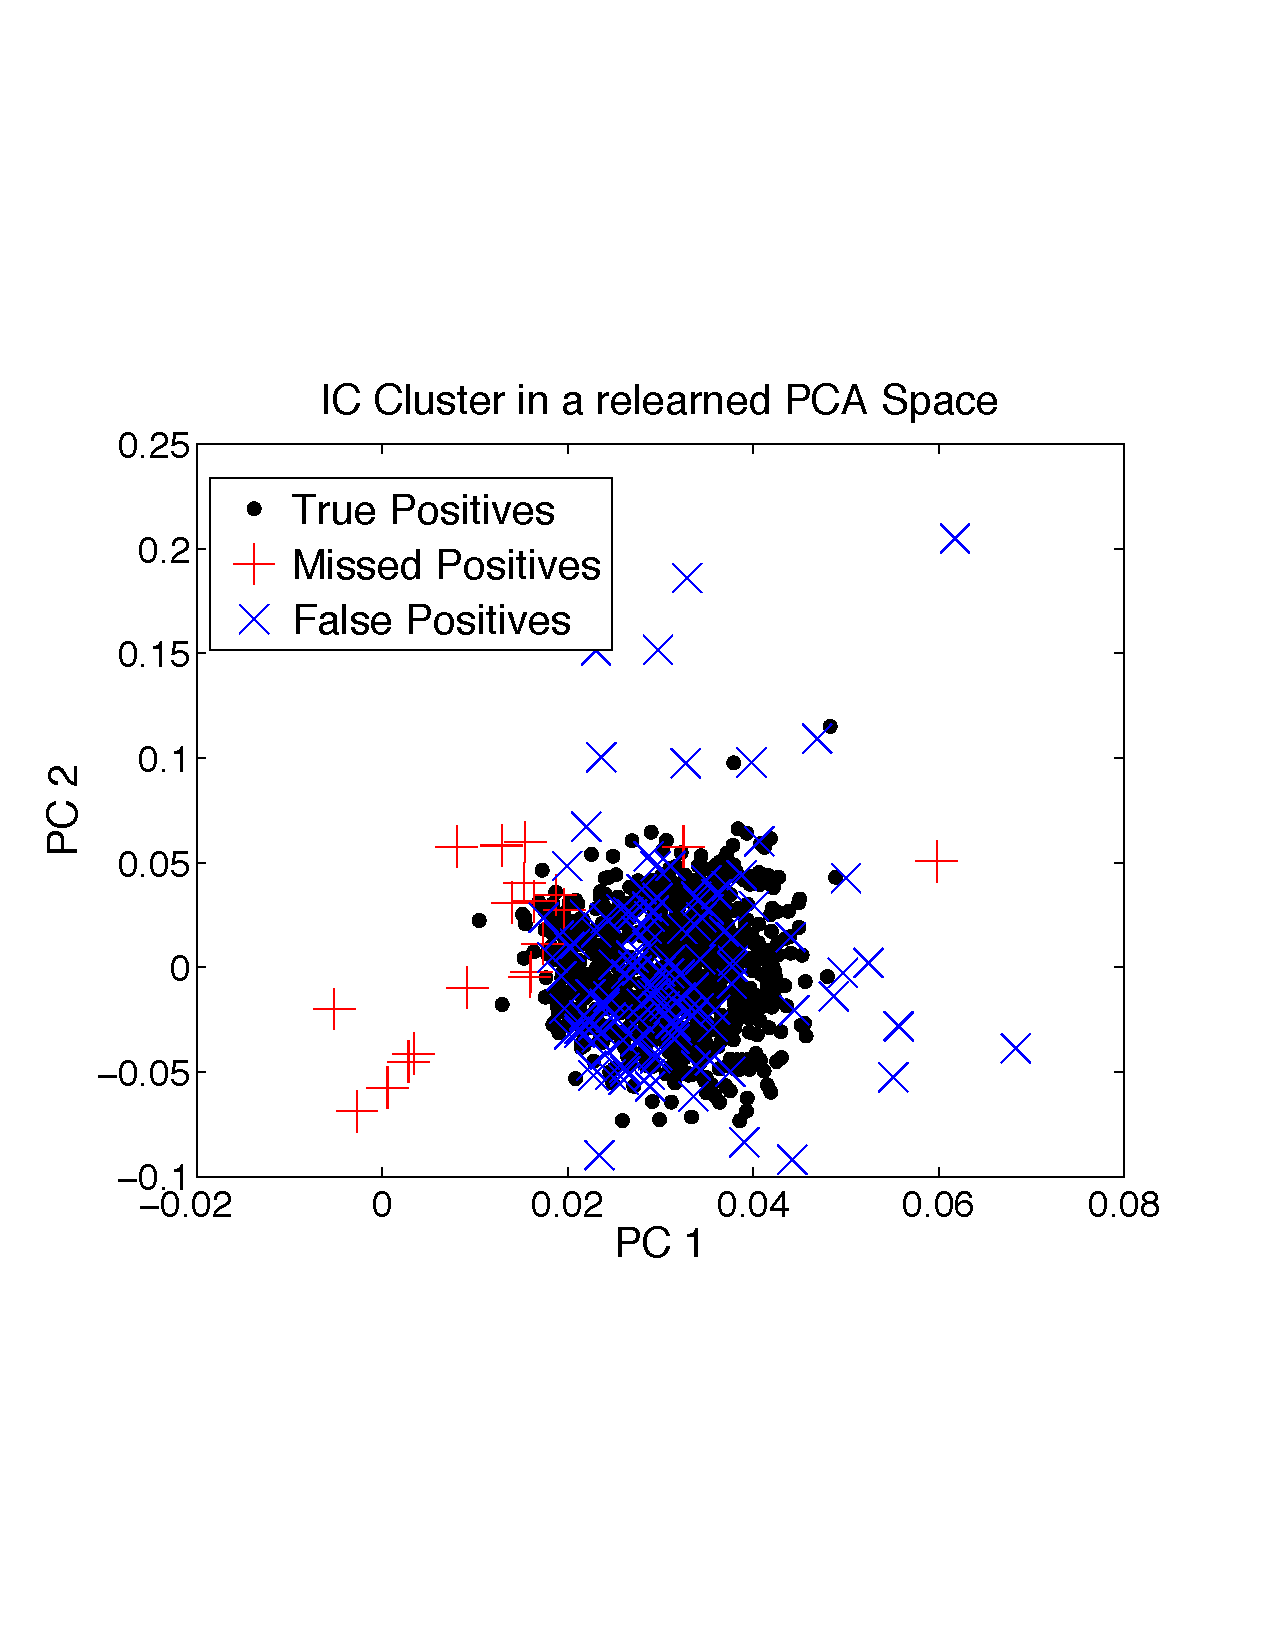
\includegraphics[width=\textwidth]{../figs/new/ICclusternewpca.pdf}
\caption{}
\label{fig:ICnew}
\end{subfigure}
\begin{subfigure}[b]{.33\textwidth}
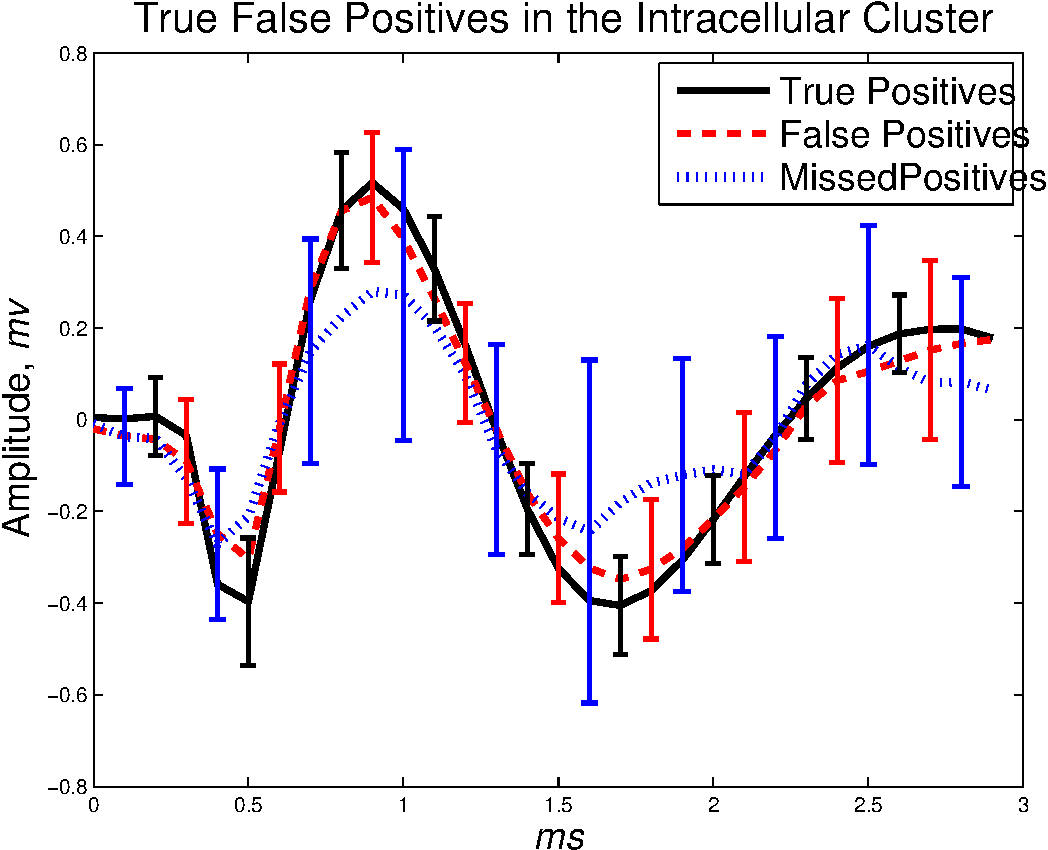
\includegraphics[width=\textwidth]{../figs/IntracellularTrueFalsePositivesv2}
\caption{}
\label{truewaveforms}
\end{subfigure}
\caption{Template matching.
(c) Errorbar plots of the true positives and the false positives in the IC cluster.  While the false positives have slightly more variability, the mean shape for the false positives and the true positives is nearly identical.  The true misses have a significantly lower amplitude as well as high variability. 
} \label{fig:IC-PCA}
\end{figure}
\end{center}

















